\part{Equipment}

\chapter{Superconducting Solenoidal Magnet}
\label{chap:eq_magnet}

\begin{figure}[htbp]
  \centering
  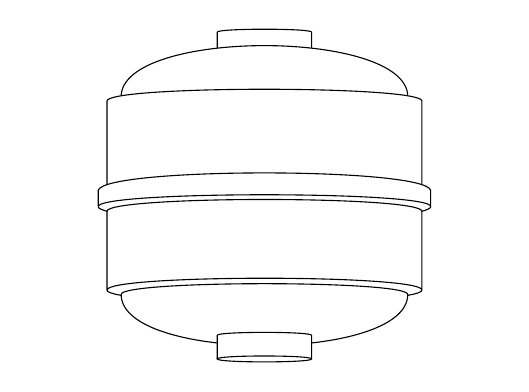
\begin{tikzpicture}
    %%%% North Endcap %%%%%%%%%%%%%%%%%%%%%%%%%%%%%%%%%%%%%%%%%%%%%%%%%%%%
    \begin{scope}[yscale=-1,fill=white]
      \draw[black,xscale=0.3,yscale=0.25,yshift=-7.1cm,fill=white]
           (-2,-1.2) coordinate (a)
        -- coordinate (ab) (-2,0) coordinate (b)   
        .. coordinate (bc) controls (-2,0.2) and (2,0.2) .. (2,0) coordinate (c)
        -- (2,-1.2) coordinate (d)
        .. coordinate (de) controls (2,-1.4) and (-2,-1.4) .. (-2,-1.2) coordinate (e);
      \draw[black,xscale=0.91,yscale=0.91,yshift=-.18cm,fill=white]
           (-2,-1.2) coordinate (sea)
        .. coordinate (ad) controls (-2,-1.0) and (2,-1.0) .. (2,-1.2)
        .. coordinate (de) controls (2,-2.15) and (-2,-2.15) .. (-2,-1.2) coordinate (-2,-1.2);
    \end{scope}

    %%%% Barrel %%%%%%%%%%%%%%%%%%%%%%%%%%%%%%%%%%%%%%%%%%%%%%%%%%%%%%%%%%
    \draw[black,fill=white]
          (-2,-1.2) coordinate (a)
       -- coordinate (ab) (-2,1.2) coordinate (b) 
       .. coordinate (bc) controls (-2,1.4) and (2,1.4) .. (2,1.2) coordinate (c)
       -- (2,-1.2) coordinate (d)
       .. coordinate (de) controls (2,-1.4) and (-2,-1.4) .. (-2,-1.2) coordinate (e)
       .. coordinate (ad) controls (-2,-1.0) and (2,-1.0) .. (d);

    \draw[black,fill=white]
         (-2.11,-.13)
      -- ++(0,.2)
      .. controls (-2,.36) and (2,.36) .. (2.11,.07)
      -- ++(0,-.2);

    \draw[black,fill=white]
         (-2,-.2)
      .. controls (-2,0) and (2,0) .. ( 2,-.2)
      .. controls (3,.08) and (-3,.08) .. (-2,-.2) --cycle;

    %%%% South Endcap %%%%%%%%%%%%%%%%%%%%%%%%%%%%%%%%%%%%%%%%%%%%%%%%%%%%
    \begin{scope}
    \draw[xscale=0.91,yscale=0.91,yshift=-.18cm,fill=white]
         (-2,-1.2) coordinate (sea)
      .. coordinate (ad) controls (-2,-1.0) and (2,-1.0) .. (2,-1.2)
      .. coordinate (de) controls (2,-2.15) and (-2,-2.15) .. (-2,-1.2) coordinate (-2,-1.2);
    \draw[xscale=0.3,yscale=0.25,yshift=-7.1cm,fill=white]
         (-2,-1.2) coordinate (a)
      -- coordinate (ab) (-2,0) coordinate (b) 
      .. coordinate (bc) controls (-2,0.2) and (2,0.2) .. (2,0) coordinate (c)
      -- (2,-1.2) coordinate (d)
      .. coordinate (de) controls (2,-1.4) and (-2,-1.4) .. (-2,-1.2) coordinate (e)
      .. coordinate (ad) controls (-2,-1.0) and (2,-1.0) .. (d);
    \end{scope}
\end{tikzpicture}

  \caption{Top-down external view of Superconducting Solenoidal Magnet}
  \label{fig:eq_magnet:topdown}
\end{figure}



The laboratory at HEP houses a Type-I superconducting solenoidal (``supersolenoid'') electromagnet wired for persistent operation.  Lacking the flux-resistive characteristics of Type-II superconductors, a Type-I superconducting electromagnet is able to maintain a constant field over the course of years, rather than the weeks to months of a higher temperature Type-II supersolenoid.  However, like all known Type-I superconductors, its critical temperature lies just north of 4\,K, necessitating that it be cooled with liquid helium (LHe).  Liquid helium boils off like liquid nitrogen, but it is a strategic resource with a limited quantity available on Earth.

Similar to other small LHe cryogen systems, the supersolenoid uses a three-chamber system.  The outer chamber is under partial vaccum to insulate the interior chambers from ambient temperature.  The middle chamber is filled with liquid nitrogen to cool the interior chambers to a maximum of 78\,K.  The innermost chamber, which houses the superconducting solenoid, is filled with liquid helium.  Liquid helium comes into direct contact with the supersolenoid.

Superconducting magnets have a number of significant advantages over ferromagnetic solenoids.  Operating at high currents, they can be relatively compact compared with their ferromagnetic cousins.  Of practical benefit in the lab, their interior (where the field direction and magnitude is nearly uniform) can be empty and externally accessible, as in our lab.  Ferromagnetic solenoids must house a ferromagnetic yoke along their axis to achieve the field strengths of supersolenoids.  When wired in persistent mode, a supersolenoid requires no additional electrical power and may remain at full strength while disconnected from a power source indefinitely.  While in persistent mode, a supersolenoid's field is more stable than a ferromagnetic solenoid, which is practically advantageous when measurements must be taken over extended periods.

The caretaker of the magnet for over three years has been Al (William A. Tobias\\<wat4y@boognish.physics.virginia.edu>), whose office is in the main Physics Building.  He has written a procedure for liquid helium fills.
%% Talk to Al, who's in the Beam (physics) building.  Caretaker of magnet for 3+ years.
%% Full address: William A. Tobias <wat4y@boognish.physics.virginia.edu>

\section{Cryogen System}
\label{sec:op_magnet:cryogens}

Maintenance of the superconductor's cryogen system is detailed in \secnameref{sec:op_maintenance}.  The cryogens boil off, and need to be monitored regularly, as detailed in \secnameref{sec:op_maintenance:cryogen_levels}.

\subsection{Liquid Nitrogen}
\label{sec:op_magnet:cryogens:ln2}

The liquid nitrogen boils off at a rate of 10\,\% per day when it is nearly full.  The rate increases somewhat as the tank approaches empty.  It's generally good policy to keep the LN2 level as high as possible, filling on Mondays and Fridays in case a fill must be missed for some reason.

The liquid nitrogen is usually delivered in 240\,L dewars, such as the Taylor-Wharton XL-65 dewar.  For filling instructions, see \secnameref{sec:op_maintenance:filling_ln2}.

\subsection{Liquid Helium}
\label{sec:op_magnet:cryogens:lhe}

The liquid helium boils off at a rate of 10\,\% per week.  One full 250\,L liquid helium dewar will fill the magnet's tank from 20\,\% to around 95\,\%.  For filling instructions, see \secnameref{sec:op_maintenance:filling_lhe}.


\section{Warnings}
\label{sec:eq_magnet}


\begin{avoid} proximity to the magnet if you carry medical equipment, including remote monitors and pacemakers.\end{avoid}

\begin{avoid} contact with the outer casing while the high voltage is active.  The central cavity of the magnet houses high voltage equipment.  Although the outer casing of the magnet \textit{should not} carry an electric potential, improper grounding, wiring, or cable failure may occur.  The high voltage to this equipment should be powered down before touching the outer casing of the magnet or the rig.\end{avoid}

\begin{avoid} bringing magnetic materials near the magnet.  The strength of the magnetic field grows inversely to the \textit{cube} of distance---that is, much faster than intuition may suggest.  Screwdrivers, metallic watches, and even metal glasses have been known to be pulled off of individuals passing by the magnet.  \textit{Remember to remove your wallet before approaching the 10\,000~gauss line near the magnet}, because it \textit{will} erase your credit cards.\end{avoid}


%%% Local Variables: 
%%% mode: latex
%%% TeX-master: "Manual"
%%% End: 
